\documentclass{article}

\usepackage{graphicx}
\usepackage{tikz}
\usepackage{tikzsymbols}
\usetikzlibrary{calc,patterns,shapes.geometric}
\pagestyle{empty}
\usepackage[margin=0pt]{geometry}
\geometry{papersize={14in,12in}}

\def\centerarc[#1](#2)(#3:#4:#5){\draw[#1] ($(#2)+({#5*cos(#3)},{#5*sin(#3)})$) arc (#3:#4:#5);}

\begin{document}
	\begin{figure}
		\centering
		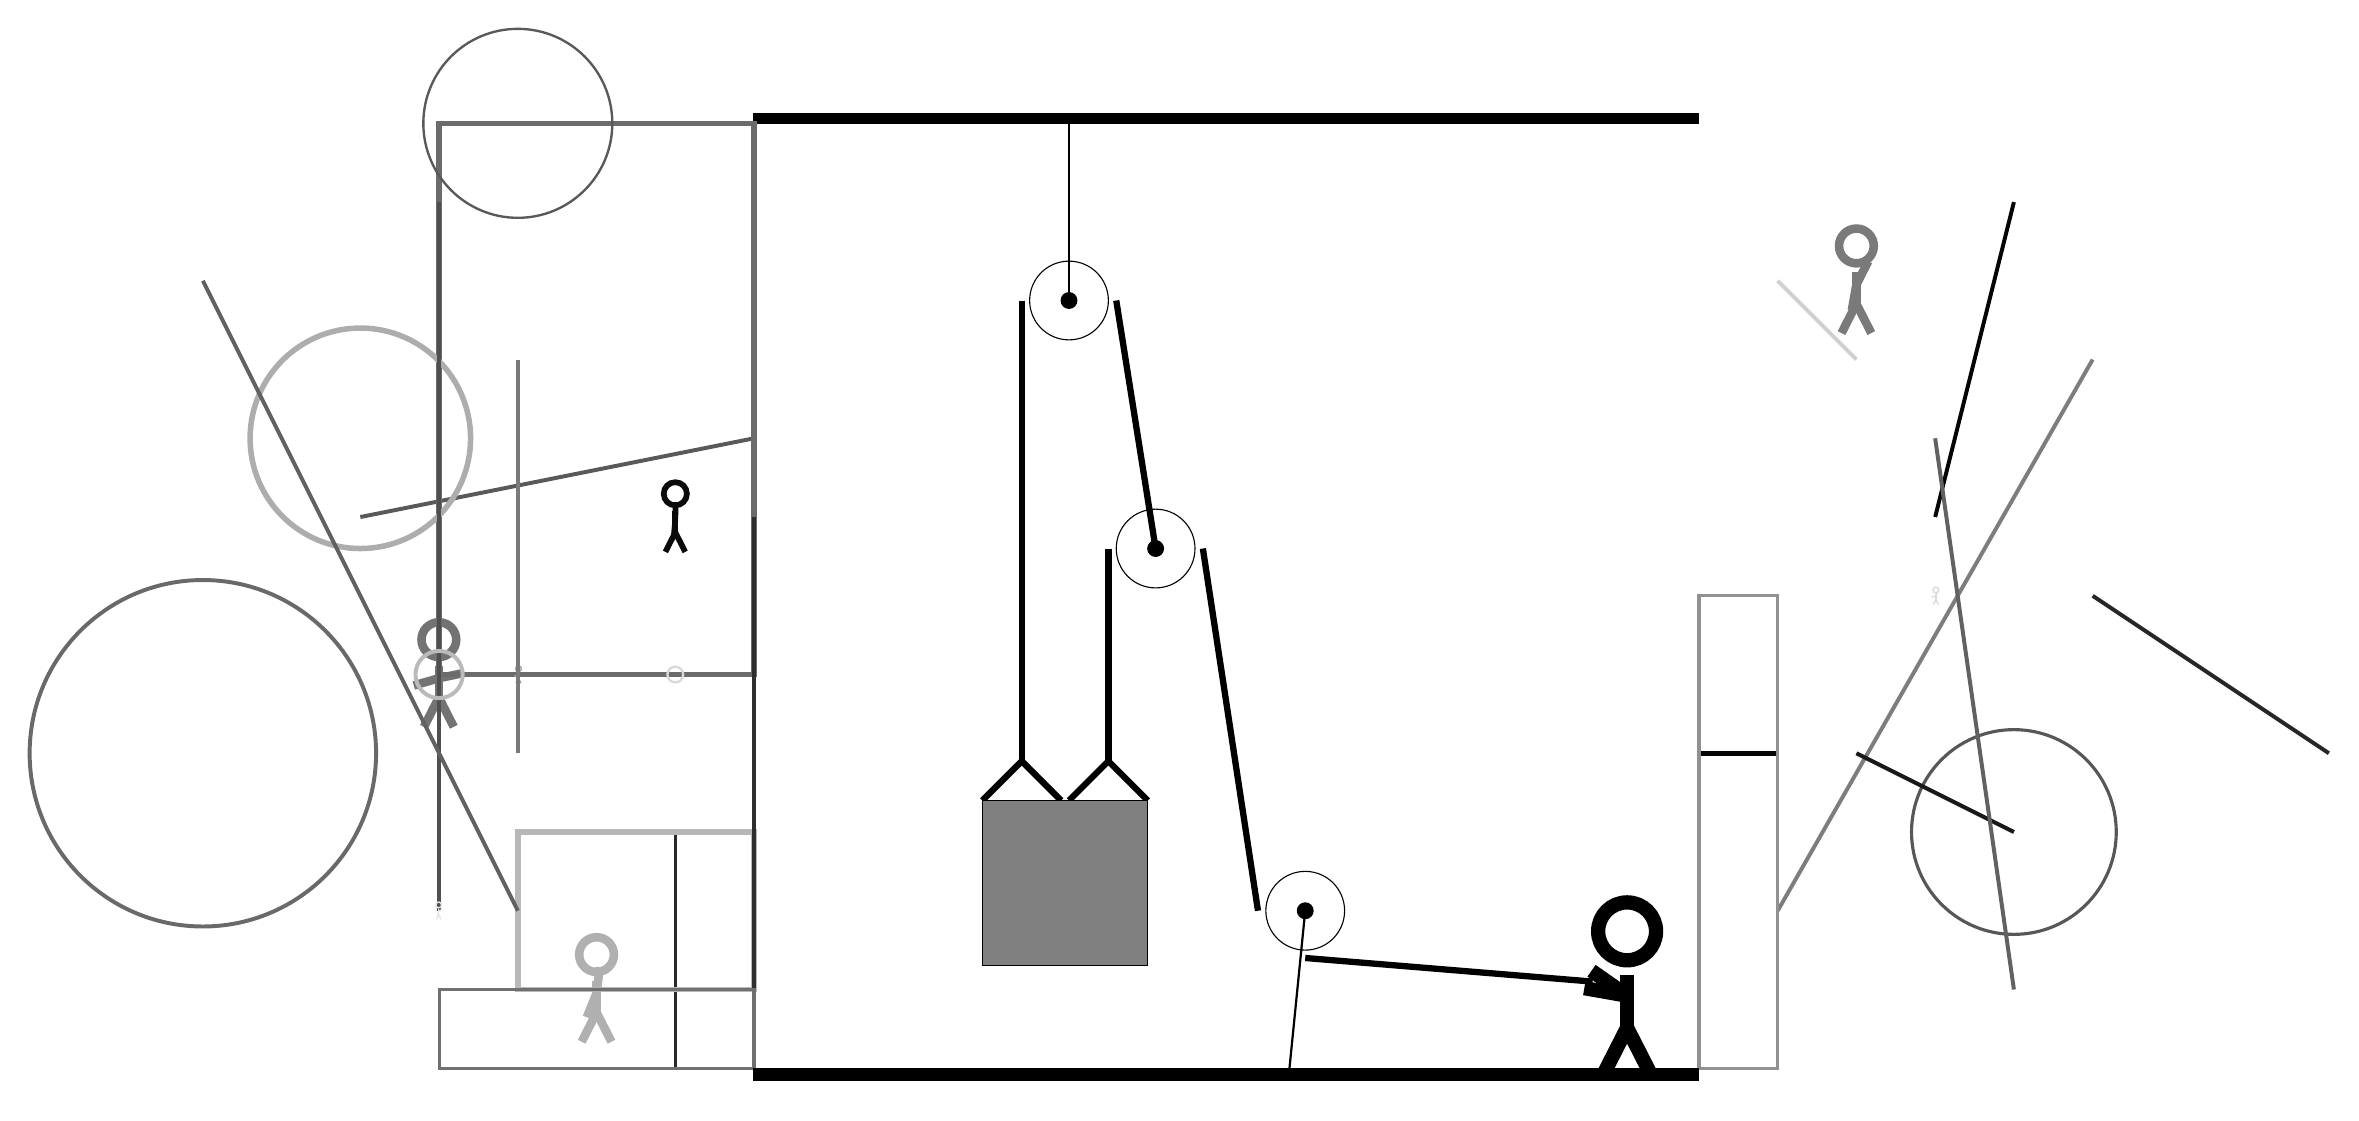
\begin{tikzpicture}
			%%%%% START %%%%%
			
			\draw[fill=black] (-2, 9) rectangle (10, 9.125);
			
			\draw (2, 6.75) circle (0.5);
			\draw[fill=black] (2, 6.75) circle (0.1);
			\draw[thick] (2, 6.75) -- (2, 9);
			
			\draw[line width=0.5mm, color=black!51](11, -1) -- (15, 6);
			
			\node[line width=0.4mm, color=black!55] at (-6, 2) {\Strichmaxerl[6][16][12]};
			\node[line width=0.4mm, color=black!14] at (13, 3) {\Strichmaxerl[1][5][73]};
			\draw[line width=0.5mm, color=black!65](-7, 4) -- (-2, 5);
			\draw [line width=0.4mm, color=black!66](14, 0) circle (1.3);
			\draw[line width=0.7mm, color=black!58] (-2, 2) rectangle (-6, 9);
			
			\draw [line width=0.3mm, color=black!65](-5, 9) circle (1.2);
			
			\draw [line width=0.7mm, color=black!32](-7, 5) circle (1.4);
			\draw[line width=0.4mm, color=black!84] (-3, -3) rectangle (-3, 0);
			\node[line width=0.6mm, color=black!36] at (-5, 2) {\Strichmaxerl[1][12][85]};
			\draw[line width=0.5mm, color=black!85](15, 3) -- (18, 1);
			\draw[line width=0.5mm, color=black!18](11, 7) -- (12, 6);
			\draw[line width=0.7mm, color=black!28] (-2, 0) rectangle (-5, -2);
			
			\draw[line width=0.5mm, color=black!98](14, 8) -- (13, 4);
			\draw [line width=0.5mm, color=black!59](-9, 1) circle (2.2);
			\draw[line width=0.5mm, color=black!69](-6, -1) -- (-6, 8);
			\draw [line width=0.3mm, color=black!15](-3, 2) circle (0.1);
			\draw[line width=0.7mm, color=black!98] (10, 1) rectangle (11, 1);
			\node[line width=0.4mm, color=black!96] at (-3, 4) {\Strichmaxerl[4][85][89]};
			\node[line width=0.5mm, color=black!10] at (-6, -1) {\Strichmaxerl[1][77][31]};
			\node[line width=0.5mm, color=black!31] at (-4, -2) {\Strichmaxerl[6][68][83]};
			\draw[line width=0.5mm, color=black!52](-5, 6) -- (-5, 1);
			\draw[line width=0.5mm, color=black!82] (-2, 4) rectangle (-2, -2);
			\node[line width=0.7mm, color=black!52] at (12, 7) {\Strichmaxerl[6][80][63]};
			\draw[line width=0.5mm, color=black!90](12, 1) -- (14, 0);
			
			\draw[line width=0.5mm, color=black!62](14, -2) -- (13, 5);
			\draw[line width=0.4mm, color=black!56] (-2, -2) rectangle (-6, -3);
			\draw [line width=0.5mm, color=black!27](-6, 2) circle (0.3);
			\draw[line width=0.5mm, color=black!62](-5, -1) -- (-9, 7);
			\draw[line width=0.4mm, color=black!43] (11, 3) rectangle (10, -3);
			
			\draw (3.1, 3.6) circle (0.5);
			\draw[fill=black] (3.1, 3.6) circle (0.1);
			
			\draw (5, -1) circle (0.5);
			\draw[fill=black] (5, -1) circle (0.1);
			\draw[thick] (5, -1) -- (4.8, -3);
			
			\draw[line width = 0.8mm]  (0.9, 0.4) -- (1.4, 0.9) -- (1.9, 0.4);
			\draw[line width = 0.8mm]  (2.0, 0.4) -- (2.5, 0.9) -- (3.0, 0.4);
			\draw[fill=black!50] (0.9, 0.4) rectangle (3.0, -1.7);
			
			\draw[line width = 0.8mm] (1.4, 6.75) -- (1.4, 0.9);
			\centerarc[line width = 0.8mm](2, 6.75)(0:180:0.6);
			\draw[line width = 0.8mm] (2.6, 6.75) -- (3.1, 3.6);
			\draw[line width = 0.8mm] (2.5, 3.6) -- (2.5, 0.9);
			\centerarc[line width = 0.8mm](3.1, 3.6)(0:180:0.6);
			\draw[line width = 0.8mm] (3.7, 3.6) -- (4.4, -1);
			\centerarc[line width = 0.8mm](5, -1)(180:270:0.6);
			\draw[line width = 0.8mm] (5, -1.6) -- (8.65, -1.9);
			
			\node at (9, -2) {\Strichmaxerl[10][-35][170]};
			
			\draw[fill=black] (-2, -3) rectangle (10, -3.15);
			
			%%%%% END %%%%%
		\end{tikzpicture}
	\end{figure}	
\end{document}